\documentclass[../main.tex]{subfiles}
	% THE RASPBERRY PI AND THE TEST BED
\begin{document}

Talk about the RPi.

%%%%%%%%%%%%%%%%%%%%%%%%%%%%%%%%%%%%%%%%%%%%%%%%%%%%%%%%%%%%%%%%%%%%%%%%%%%%%%%%%%%%%%%%%%%%%%%%%%%%%%%%%%%%%%%%%%%%%%%%%%%%%%%%%%

\section{Fundamentals}

The Raspberry Pi is a simple, affordable ARM-based computing module. It has, which can interface\\

It is run using a Linux-based operating system called Raspbian which is available for download from the Raspberry Pi official website \ref{web_Raspbian}.\\

\subsection{Blablabla}
Talky talk talk

%%%%%%%%%%%%%%%%%%%%%%%%%%%%%%%%%%%%%%%%%%%%%%%%%%%%%%%%%%%%%%%%%%%%%%%%%%%%%%%%%%%%%%%%%%%%%%%%%%%%%%%%%%%%%%%%%%%%%%%%%%%%%%%%%%
	
\section{Test Bed Architecture}

The test bed comprises the two Raspberry Pis and a number of chips to provide the functions required for more advanced modulation schemes.
This is built up as three arrangements with increasing complexity.
The first is the Pis connected together by two wires, a serial data line and a clock line (Figure \ref{fig_OOK Architecture}).
This arrangement is similar to that used for an $I^2C$ bus, however the code written for this form of communication doesn't rely on any available modes of serial interfacing because it needs to be extensible to the parallel communication in the next arrangements.
The second arrangement is used for Pulse Amplitude Modulation schemes.
It uses a single parallel Digital Analogue Converter (DAC) connected to the transmitter which transmits to a parallel Analogue Digital Converter connected to the receiver, allowing for multi-level signals to be transmitted between the two devices.
The final arrangement extends the set-up to two DACs and two ADCs.
These signals are then multiplied by a sine wave and a cosine wave respectively, and can be separated due to the orthogonality of the two signals at the receiver.
This arrangement is used for Quadrature Amplitude Modulation as well as Orthogonal Frequency Division Multiplexing.\\

\missingfigure{Test Bed Set-up For On-Off Keying}

\begin{figure}[ht]
	\centering
	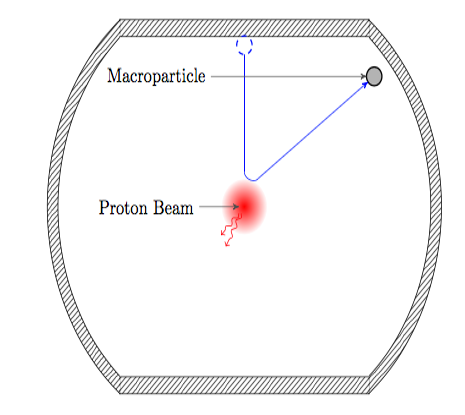
\includegraphics[width=0.6\textwidth]{UFO_Falling.png}
	\caption{Test Bed Set-up For On-Off Keying}
	\label{fig_OOK Architecture}
\end{figure}

\subsection{Digital Analogue Converter}

The Digital Analogue Converter used is the AD5424, 

\subsection{Analogue Digital Converter}

The Digital Analogue Converter used is the AD5424, 

\subsection{Parts Used}

It is worth noting that there is a large variety of available options for each component of the test bed.
Each possibility has certain advantages and disadvantages, and a lot of the options are not suitable due to the power requirements or ease of interfacing with the Raspberry Pi.
As a result of this, the parts used in this project were the most suitable parts which could be found and successfully sourced.
However, there may be more suitable chips available given more time or experience, and being aware of this would be useful if this project were to be extended and/or replicated.\\

Changes which would be made with hindsight, if components with the required qualities could be found, are as follows:

\todo[inline,color=blue!20]{Continue to add to this list as you write the Architecture section - remove redundant information already discussed in earlier sections}
\begin{itemize}
	\item A number of chips used are surface mounted, requiring difficult soldering to solder pads, This would be useful if they were to be used on a printed circuit board for a final design, but on a prototyping breadboard, dual in-line packages would have been easier to use where available
	\item The Digital Analogue Converter was chosen for its easy interfacing with a microcontroller, but a voltage-output device would remove the need to use additional operational amplifiers at the output
	\item Analogue Digital Converter
	\item The Quadrature Sinusoid Generator uses an oscillator chip which outputs $90^o$ out-of-phase square waves, and the used chip was the only simple one which did this. Ideally the outputs would already be sinusoidal (one quadrature chip or a sine generator and phase shifter) so that low pass filters with fixed frequency response could be omitted to make changing the carrier frequency purely software-dependent.
	\todo[inline]{Make sure I am consistent with use of Quadrature Sinusoid Generator vs Oscillator in report}	
	\item The multiplier is designed to operate around \SI{10}{\volt}, and so has a built in \SI{10}{\volt} normalisation in the multiple which attenuates the signal and required re-amplification before transmission. A similar chip designed for lower voltages would be ideal.
	\todo[inline]{Fact check this}
	\item Low Pass Filters
\end{itemize}

%%%%%%%%%%%%%%%%%%%%%%%%%%%%%%%%%%%%%%%%%%%%%%%%%%%%%%%%%%%%%%%%%%%%%%%%%%%%%%%%%%%%%%%%%%%%%%%%%%%%%%%%%%%%%%%%%%%%%%%%%%%%%%%%%%

\section{Programming}

The Raspberry Pi is used for its low cost, ease of use, and the fact that it has programmable Input/Output (I/O) pins.
The I/O pins can be programmed using different libraries in Python and C.
The standard library which comes installed with Raspbian is the RPi.GPIO Python library \ref{web_RPi.GPIO}.
\todo[inline,color=green!40]{Add bib reference to RPi.GPIO https://pypi.python.org/pypi/RPi.GPIO}
This is used for the On-Off Keying part of the communications test bed, and then a C library is used for the pin-level manipulation for all modulation schemes requiring multi-level outputs through Digital Analogue Converters.
This is for the improved speed performance of the C library and for the capability of this library to output to multiple pins at once.
Section \ref{sec_Comparing Python and C} goes into a detailed  investigation of the differences between these options.
All of the code and the report for the project are maintained on GitHub, and may be found at \url{https://github.com/CamEadie/4YP_PiCom}.\\

The code is separated into the initial On-Off Keying (Section \ref{sec_On-Off Keying}) which acts as a proof of concept for the Raspberry Pis as a test bed, and the Advanced Modulation Schemes (Section \ref{sec_Advanced Modulation Schemes}) which are all implemented in the same code.
The Advanced section improves the data manipulation and implements a separate compiled module for the actual transmitting and receiving of data.

\subsection{On-Off Keying} \label{sec_On-Off Keying}

\subsubsection{Starting the Receiver}
\todo[inline]{Paramiko}

\subsection{Advanced Modulation Schemes} \label{sec_Advanced Modulation Schemes}

\subsubsection{Data and Image Handling}
\subsubsection{C Transmitter and Receiver}

\end{document}